\chapter{Bloc II : Probabilitat i estadística}

\section{Probabilitat}
\subsection{Distribució normal}

\subsubsection{Què és la distribució normal?}
Imagina’t que mesures l’alçada de tots els alumnes del teu curs. La majoria estaran a prop de l’alçada mitjana (ni molt alts ni molt baixos), però a mesura que et vas allunyant més d’aquesta mitjana (molt alt o molt baix) menys gent trobes. Si dibuixes aquestes alçades en un gràfic surt una corba en forma de campana, coneguda com a campana de Gauss.
Doncs la distribució normal és el model matemàtic d’aquesta campana.

\begin{figure}[h!]
    \centering
    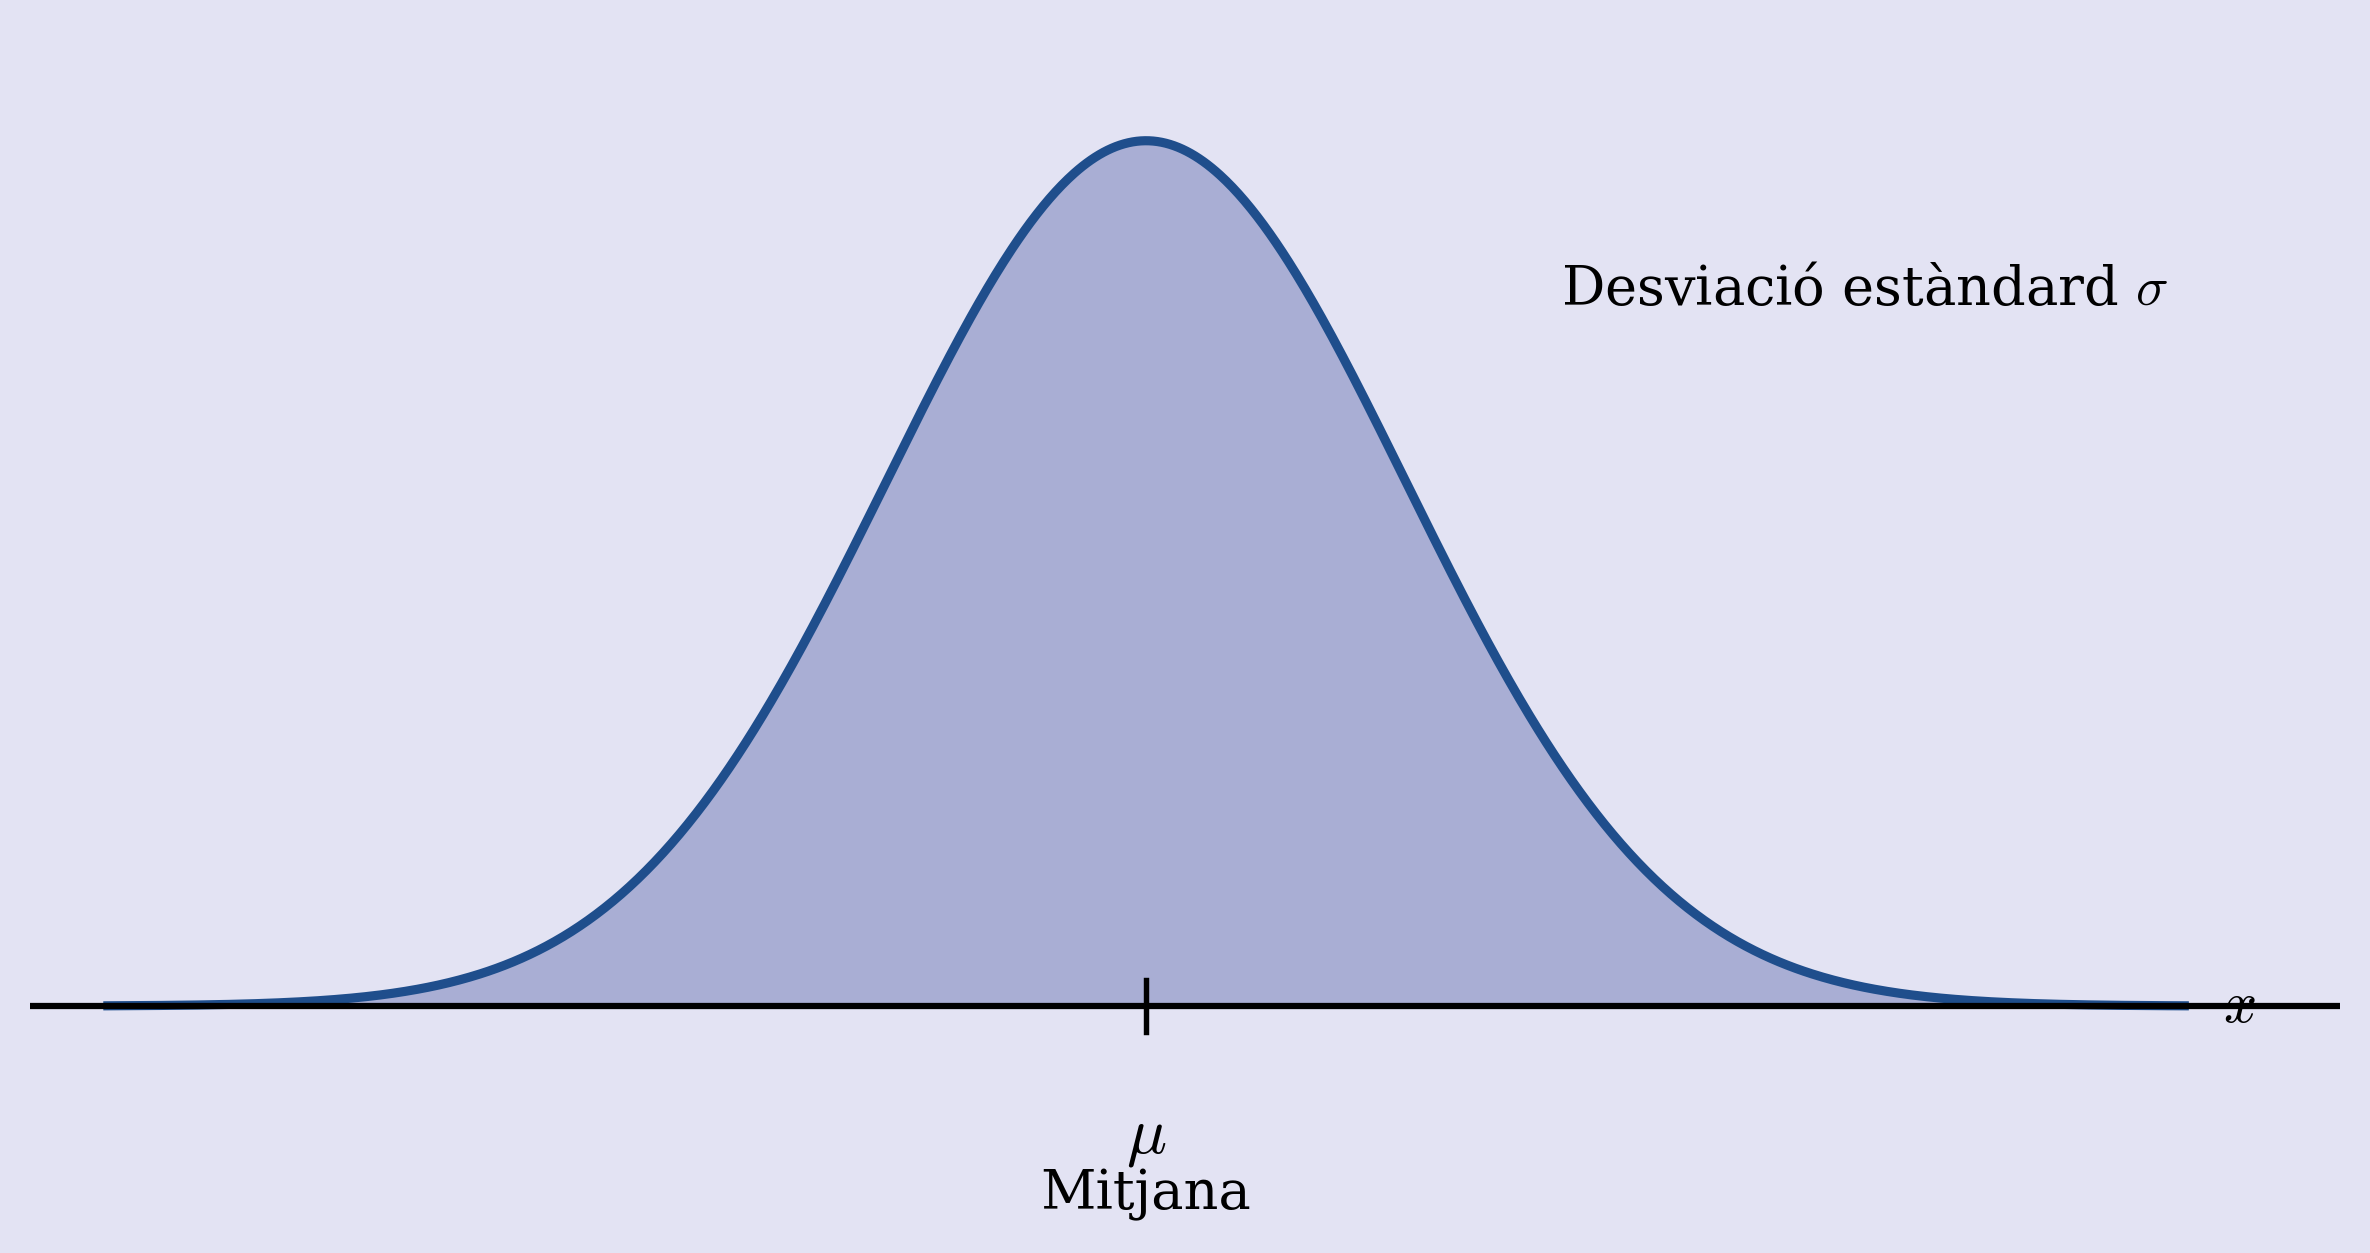
\includegraphics[width=0.7\textwidth]{./figures/distribucio_normal.png}
    \caption{Distribució normal amb mitjana $\mu$ i desviació típica $\sigma$}
\end{figure}


\subsubsection{Definició i paràmetres}
La distribució normal s’expressa com: $X \sim N(\mu, \sigma)$, on $\mu$ és la mitjana i $\sigma$ la desviació típica~\ref{desviació-típica}. Visualment, $\mu$ marca el centre de la campana, mentre que $\sigma$ determina l'amplada: com més gran és $\sigma$, més ampla és la campana i com més petita és, més estreta.

La versió estàndard per mirar les probabilitats és quan $Z \sim N(0,1)$, perquè les taules de probabilitat estan fetes per a aquesta distribució. Tot i que, a les PAU de Catalunya no és necessari utilitzar aquestes taules, ja que en l’enunciat et donen directament la probabilitat.

En el cas que la variable no segueixi la distribució $N(0,1)$, es pot transformar en una distribució normal estàndard mitjançant la tipificació: $Z = \frac{X - \mu}{\sigma}$.


\begin{table}[h!]
    \centering
    \begin{scriptsize}
     \begin{tabular}{c|cccccccccc}
        \hline
        z & 0.00 & 0.01 & 0.02 & 0.03 & 0.04 & 0.05 & 0.06 & 0.07 & 0.08 & 0.09 \\
        \hline
                0.0 & 0.5000 & 0.5040 & 0.5080 & 0.5120 & 0.5160 & 0.5199 & 0.5239 & 0.5279 & 0.5319 & 0.5359 \\
        0.1 & 0.5398 & 0.5438 & 0.5478 & 0.5517 & 0.5557 & 0.5596 & 0.5636 & 0.5675 & 0.5714 & 0.5753 \\
        0.2 & 0.5793 & 0.5832 & 0.5871 & 0.5910 & 0.5948 & 0.5987 & 0.6026 & 0.6064 & 0.6103 & 0.6141 \\
        0.3 & 0.6179 & 0.6217 & 0.6255 & 0.6293 & 0.6331 & 0.6368 & 0.6406 & 0.6443 & 0.6480 & 0.6517 \\
        0.4 & 0.6554 & 0.6591 & 0.6628 & 0.6664 & 0.6700 & 0.6736 & 0.6772 & 0.6808 & 0.6844 & 0.6879 \\
        0.5 & 0.6915 & 0.6950 & 0.6985 & 0.7019 & 0.7054 & 0.7088 & 0.7123 & 0.7157 & 0.7190 & 0.7224 \\
        0.6 & 0.7257 & 0.7291 & 0.7324 & 0.7357 & 0.7389 & 0.7422 & 0.7454 & 0.7486 & 0.7517 & 0.7549 \\
        0.7 & 0.7580 & 0.7611 & 0.7642 & 0.7673 & 0.7704 & 0.7734 & 0.7764 & 0.7794 & 0.7823 & 0.7852 \\
        0.8 & 0.7881 & 0.7910 & 0.7939 & 0.7967 & 0.7995 & 0.8023 & 0.8051 & 0.8078 & 0.8106 & 0.8133 \\
        0.9 & 0.8159 & 0.8186 & 0.8212 & 0.8238 & 0.8264 & 0.8289 & 0.8315 & 0.8340 & 0.8365 & 0.8389 \\
        1.0 & 0.8413 & 0.8438 & 0.8461 & 0.8485 & 0.8508 & 0.8531 & 0.8554 & 0.8577 & 0.8599 & 0.8621 \\
        1.1 & 0.8643 & 0.8665 & 0.8686 & 0.8708 & 0.8729 & 0.8749 & 0.8770 & 0.8790 & 0.8810 & 0.8830 \\
        1.2 & 0.8849 & 0.8869 & 0.8888 & 0.8907 & 0.8925 & 0.8944 & 0.8962 & 0.8980 & 0.8997 & 0.9015 \\
        1.3 & 0.9032 & 0.9049 & 0.9066 & 0.9082 & 0.9099 & 0.9115 & 0.9131 & 0.9147 & 0.9162 & 0.9177 \\
        1.4 & 0.9192 & 0.9207 & 0.9222 & 0.9236 & 0.9251 & 0.9265 & 0.9279 & 0.9292 & 0.9306 & 0.9319 \\
        1.5 & 0.9332 & 0.9345 & 0.9357 & 0.9370 & 0.9382 & 0.9394 & 0.9406 & 0.9418 & 0.9429 & 0.9441 \\
        1.6 & 0.9452 & 0.9463 & 0.9474 & 0.9484 & 0.9495 & 0.9505 & 0.9515 & 0.9525 & 0.9535 & 0.9545 \\
        1.7 & 0.9554 & 0.9564 & 0.9573 & 0.9582 & 0.9591 & 0.9599 & 0.9608 & 0.9616 & 0.9625 & 0.9633 \\
        1.8 & 0.9641 & 0.9649 & 0.9656 & 0.9664 & 0.9671 & 0.9678 & 0.9686 & 0.9693 & 0.9699 & 0.9706 \\
        1.9 & 0.9713 & 0.9719 & 0.9726 & 0.9732 & 0.9738 & 0.9744 & 0.9750 & 0.9756 & 0.9761 & 0.9767 \\
        2.0 & 0.9772 & 0.9778 & 0.9783 & 0.9788 & 0.9793 & 0.9798 & 0.9803 & 0.9808 & 0.9812 & 0.9817 \\
        2.1 & 0.9821 & 0.9826 & 0.9830 & 0.9834 & 0.9838 & 0.9842 & 0.9846 & 0.9850 & 0.9854 & 0.9857 \\
        2.2 & 0.9861 & 0.9864 & 0.9868 & 0.9871 & 0.9875 & 0.9878 & 0.9881 & 0.9884 & 0.9887 & 0.9890 \\
        2.3 & 0.9893 & 0.9896 & 0.9898 & 0.9901 & 0.9904 & 0.9906 & 0.9909 & 0.9911 & 0.9913 & 0.9916 \\
        2.4 & 0.9918 & 0.9920 & 0.9922 & 0.9925 & 0.9927 & 0.9929 & 0.9931 & 0.9932 & 0.9934 & 0.9936 \\
        2.5 & 0.9938 & 0.9940 & 0.9941 & 0.9943 & 0.9945 & 0.9946 & 0.9948 & 0.9949 & 0.9951 & 0.9952 \\
        2.6 & 0.9953 & 0.9955 & 0.9956 & 0.9957 & 0.9959 & 0.9960 & 0.9961 & 0.9962 & 0.9963 & 0.9964 \\
        2.7 & 0.9965 & 0.9966 & 0.9967 & 0.9968 & 0.9969 & 0.9970 & 0.9971 & 0.9972 & 0.9973 & 0.9974 \\
        2.8 & 0.9974 & 0.9975 & 0.9976 & 0.9977 & 0.9977 & 0.9978 & 0.9979 & 0.9979 & 0.9980 & 0.9981 \\
        2.9 & 0.9981 & 0.9982 & 0.9982 & 0.9983 & 0.9984 & 0.9984 & 0.9985 & 0.9985 & 0.9986 & 0.9986 \\
        3.0 & 0.9987 & 0.9987 & 0.9987 & 0.9988 & 0.9988 & 0.9989 & 0.9989 & 0.9989 & 0.9990 & 0.9990 \\
        3.1 & 0.9990 & 0.9991 & 0.9991 & 0.9991 & 0.9992 & 0.9992 & 0.9992 & 0.9992 & 0.9993 & 0.9993 \\
        3.2 & 0.9993 & 0.9993 & 0.9994 & 0.9994 & 0.9994 & 0.9994 & 0.9994 & 0.9995 & 0.9995 & 0.9995 \\
        3.3 & 0.9995 & 0.9995 & 0.9995 & 0.9996 & 0.9996 & 0.9996 & 0.9996 & 0.9996 & 0.9996 & 0.9997 \\
        3.4 & 0.9997 & 0.9997 & 0.9997 & 0.9997 & 0.9997 & 0.9997 & 0.9997 & 0.9997 & 0.9997 & 0.9998 \\
        3.5 & 0.9998 & 0.9998 & 0.9998 & 0.9998 & 0.9998 & 0.9998 & 0.9998 & 0.9998 & 0.9998 & 0.9998 \\
        3.6 & 0.9998 & 0.9998 & 0.9999 & 0.9999 & 0.9999 & 0.9999 & 0.9999 & 0.9999 & 0.9999 & 0.9999 \\
        3.7 & 0.9999 & 0.9999 & 0.9999 & 0.9999 & 0.9999 & 0.9999 & 0.9999 & 0.9999 & 0.9999 & 0.9999 \\
        3.8 & 0.9999 & 0.9999 & 0.9999 & 0.9999 & 0.9999 & 0.9999 & 0.9999 & 0.9999 & 0.9999 & 0.9999 \\
        3.9 & 1.0000 & 1.0000 & 1.0000 & 1.0000 & 1.0000 & 1.0000 & 1.0000 & 1.0000 & 1.0000 & 1.0000 \\
        \hline
    \end{tabular}
    \end{scriptsize}
    \caption{Taula de la distribució normal estàndard N(0,1)}
    \label{tau-normal}
\end{table}


\subsubsection{Exercicis resolts}
Exercici 1:
Enunciat: Si $Z \sim N(0,1)$, calcula $P(Z<1,45)$.
\begin{figure}[h!]
    \centering
    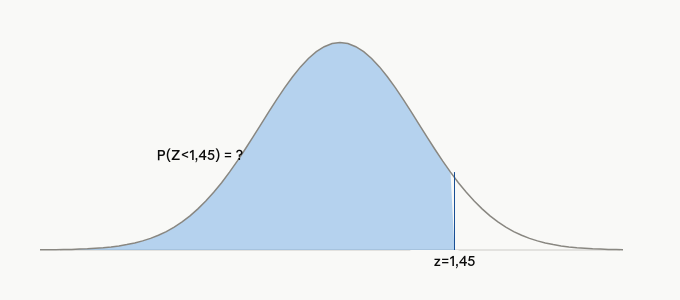
\includegraphics[width=0.8\textwidth]{./figures/Exercici_resolt_1.png}
    \caption{Àrea corresponent a $P(Z<1,45)$ sota la corba normal estàndard.}
\end{figure}

Resolució:
La taula~\ref{tau-normal} de la dona directament l'àrea acumulada a l'esquerra de $Z \sim N(0,1)$ (la probabilitat que necessitem calcular). Només cal buscar la fila 1,4 i la columna 0,05 (per formar 1,45):
$P(Z<1,45)=0.9265$
No cal cap càlcul previ: la taula ja et dona la probabilitat acumulada fins a aquell valor.

Exercici 2:
Enunciat: Si $Z \sim N(0,1)$, calcula $P(Z>0,8)$.
\begin{figure}[h!]
    \centering
    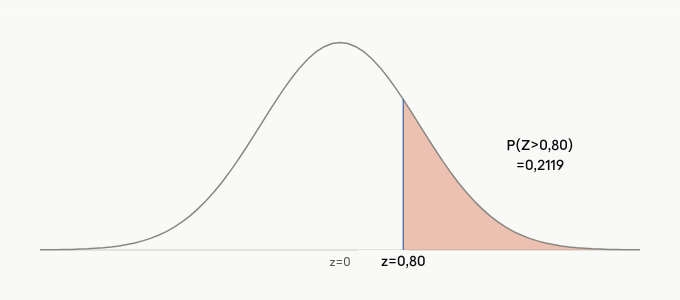
\includegraphics[width=0.8\textwidth]{./figures/Exercici_resolt_2.png}
    \caption{Àrea corresponent a $P(Z>0,8)$ sota la corba normal estàndard.}
\end{figure}

Resolució:
La taula només dona probabilitats acumulades "menys que". Com que tota l'àrea sota la corba val 1:
$P(Z>0,8)=1-P(Z<0,8)=1-0,7881=0,2119$
Idea clau: sempre que et demanin ``més gran que'', passau a ``1 menys la probabilitat de la taula''

Exercici 3:
Enunciat: Si $Z \sim N(0,1)$, calcula $P(-1<Z<1,5)$.
\begin{figure}[h!]
    \centering
    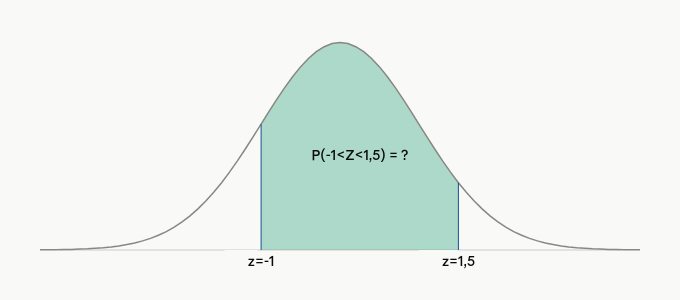
\includegraphics[width=0.8\textwidth]{./figures/Exercici_resolt_3.png}
    \caption{Àrea corresponent a $P(-1<Z<1,5)$ sota la corba normal estàndard.}
\end{figure}

Resolució:
Aquí et donen un interval, així que és la resta de dues àrees acumulades (és la àrea acumulada del número més gran, $1,5$, menys la àrea del petit, $-1$):
$P(-1<Z<1,5)=P(Z<1,5)-P(Z<-1)$
Per a $Z<-1$, fem servir la simetria de la normal:
$P(Z<-1)=1-P(Z<1)=1-0,8413=0,1587$
Llavors:
$P(-1<Z<1,5)=P(Z<1,5)-P(Z<-1)=0,9332-0,1587=0,7745$
Idea clau: amb valors negatius de $z$, sempre ``els gires'' fent servir $P(Z<-z)=1-P(Z<z)$.

Exercici 4:
Enunciat: Les notes d'un examen d'una classe segueixen $X \sim N(65, 12)$. Calcula $P(X<80)$.
\begin{figure}[h!]
    \centering
    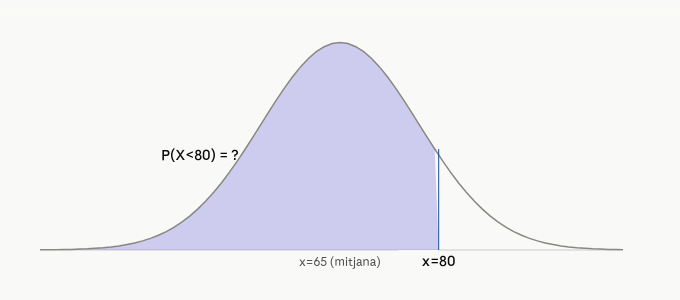
\includegraphics[width=0.7\textwidth]{./figures/Exercici_resolt_4.png}
    \caption{Àrea corresponent a $X \sim N(65, 12)$ sota la corba normal estàndard.}
\end{figure}

Resolució:
\begin{enumerate}[(1)]
 \item  Tipificar. Com que $X$ no és $N(0, 1)$, no podem mirar la taula directament amb $80$. Cal passar-ho a una $Z$ estàndard: $$Z=\frac{X - \mu}{\sigma}=\frac{80-65}{12}=1,25$$
 \item Reescriure la probabilitat en termes de $Z$ i mirar taula:
$P(X<80)=P(Z<1,25)=0,8944$
\end{enumerate}

Resposta: aproximadament el $89,44\%$ dels estudiants treuen menys de 80 punts.

\subsubsection{Exercicis a resoldre de la distribució normal:}
\begin{enumerate}
 \item Si $Z \sim N(0, 1)$, calcula $P(Z<2,1)$.
 \item Si $Z \sim N(0, 1)$, calcula $P(Z>1,33)$.
 \item Si $Z \sim N(0, 1)$, calcula $P(Z<-0,55)$.
 \item Si $Z \sim N(0, 1)$, calcula $P(-2<Z<0,5)$.
 \item Si $Z \sim N(0, 1)$, troba $z$ tal que $P(Z<z)0,95$.
 \item Si $X \sim N(40, 5)$, calcula $P(X<47)$.
 \item Si $X \sim N(120, 20)$, calcula $P(X>100)$.
 \item El temps de reacció d'un grup de conductors segueix $N(0,75, 0,12)$ segons. Quina probabilitat té un conductor que tingui un temps de reacció més gran de $0,9$ s?
 \item Les puntuacions d'un test segueixen $N(100,15)$. Quina proporció de persones obté una puntuació entre $85$ i $115$?
 \item Una variable $N(80,\sigma)$ compleix que $P(X<65)=0,05$. Calcula $\sigma$.
 \item PAU Catalunya, Matemàtiques Aplicades a les Ciències Socials, convocatòria ordinària de 2025, exercici 3a.
    Enunciat: Fa uns anys una granja de vaques frisones dedicada a la producció de llet va fer un estudi sobre el pes de les seves vaques i va arribar a la conclusió que aquesta variable seguia una distribució normal amb una mitjana de 580 kg i una desviació típica de 25 kg. Calculeu, de manera raonada, la probabilitat que si agafem a l’atzar una vaca frisona d’aquesta granja, el seu pes estigui entre 531 i 629 kg.
\end{enumerate}



\subsection{Aproximació de la binomial per la normal}
\subsubsection{Perquè aproximar-la}
Quan $n$ és gran, calcular probabilitats amb la fórmula de la binomial es torna molt feixuc (combinatòries enormes). Per evitar fer càlculs enormes aproximem la binomial per una distribució normal, que és contínua i molt més fàcil de treballar amb taules.


\subsubsection{Quan s'aplica}
En el llibre de MACS II~\cite{Llibre_MACS_II} a la pàgina 320 explica que:
\emph{Una distribució binomial s'assembla més a una de normal com més gran és el producte $np$ (o $nq$ si $q<p$)} ($q=1-p$).

\emph{Quan $np$ i $nq$ són més grans que 3, l'aproximació és bastant bona. I si són més grans que 5, l'aproximació és gairebé perfecta. D'ara endavant considerarem el valor 3 com a referent per dona validesa a aquesta aproximació.
Naturalment, la corba normal a la qual s'aproxima la $B(n, p)$ té la mateixa mitjana, $\mu = n \cdot p$, i la mateixa desviació típica, $\sigma = \sqrt{n \cdot p \cdot q}$:
$B(n, p) \approx N(n \cdot p, \sqrt{n \cdot p \cdot q}$
En l'aproximació d'ambdues distribucions cal tenir en compte que la binomial és discreta i la normal, contínua.}

\subsubsection{La correcció de continuïtat}
La binomial és discreta (només agafa valors enters), mentre que la normal és contínua (pot pendre qualsevol valor dins d'un interval, incloent-hi els tots els decimals possibles). Per passar d'una a l'altra, cal ``fer més gran'' cada valor enter k en un interval [k-0,5, k+0,5].
Taula de conversió:
\begin{table}[h!]
    \centering
    \begin{tabular}{c|c}
        \hline
        Volem (binomial) & Ho calculem amb (normal) \\
        \hline
        $P(X=k)$ & $P(k-0,5<Y<k+0,5)$ \\
        $P(X\leq k)$ & $P(Y<k+0,5)$ \\
        $P(X<k)$ & $P(Y<k-0,5)$ \\
        $P(X\geq k)$ & $P(Y>k-0,5)$ \\
        $P(X>k)$ & $P(Y>k+0,5)$ \\
        \hline
    \end{tabular}
    \caption{Correcció de continuïtat: pas de binomial a normal}
    \label{tau-correccio-continuitat}
\end{table}

\subsubsection{Exercici resolt}
Enunciat: En una fàbrica, el 8\% de les peces són defectuoses. S'agafa una mostra de 200 peces. Calcula la probabilitat que n'hi hagi com a màxim 20 de defectuoses.



Resolució:
\begin{enumerate}[(1)]
 \item Definir paràmetres i identificar la binomial: $n=200; p=0,08; q=1-0,08=0,92$ $X \sim B(200;\ 0,08)$
 \item Comprovar condicions: $np=16\geq3$, $nq=184\geq3$
 \item Calcular els paràmetres: $$\mu=16$$ $$\sigma=\sqrt{200 \cdot 0,08 \cdot 0,92}\approx 3,83$$
 \item Aplicar la correcció de continuïtat: com que volem $P(X\leq20)$, passem a $P(Y<20,5)$
 \item Tipificar: $Z=\frac{20,5-16}{3,83}\approx 1,17$
 \item Consultar la taula $N(0,1)$: $P(Z<1,17)\approx 0,8790$
\end{enumerate}

Resposta: la probabilitat que hi hagi com a màxim 20 peces defectuoses és aproximadament $87,90\%$.

\subsubsection{Exercicis a resoldre de l'aproximació de la binomial per la normal:}
\begin{enumerate}
 \item Si $X \sim B(150, 0,4)$, comprova que es pot aproximar per una normal i calcula els paràmetres $\mu$ i $\sigma$ de la normal corresponent.
 \item Si $X \sim B(300, 0,25)$, calcula $P(X \leq 80)$ aproximant per la normal.
 \item Si $X \sim B(100, 0,5)$, calcula $P(X > 55)$ aproximant per la normal.
 \item Si $X \sim B(250, 0,6)$, calcula $P(X = 150)$ aproximant per la normal.
 \item En un institut, el $65\%$ dels alumnes de batxillerat afirmen fer esport regularment. Si s'entrevisten $180$ alumnes a l'atzar, calcula la probabilitat que com a màxim $110$ facin esport regularment.
 \item En una companyia telefònica, s'ha observat que aproximadament un $12\%$ de les trucades al servei d'atenció al client duren més de $10$ minuts. D'una mostra de $400$ trucades, calcula la probabilitat que entre $40$ i $55$ (ambdós inclosos) durin més de $10$ minuts.
 \item Segons un estudi, el $30\%$ dels joves d'entre $16$ i $18$ anys practica algun esport federat. Es tria una mostra aleatòria de $120$ joves d'aquesta franja d'edat. Calcula, de manera raonada, la probabilitat que com a mínim $30$ dels joves de la mostra practiquin algun esport federat.
\end{enumerate}



\section{Inferència}
\subsection{La introducció al mostreig estadístic}
La \textbf{població} o \textbf{l'univers} és el conjunt de tots els individus o elements que formen part del nostre estudi

Una \textbf{mostra} és un subconjunt d'elements extrets d'una població més gran, que s'utilitza per estudiar les característiques d'aquesta població sense haver-la d'analitzar completament.

\subsubsection{Mostreig}
Per a que la mostra sigui el més representativa possible a la població existeixen diferents tipus de \textbf{mostreigs}. A continuació veurem com fer el mostreig perquè ens doni mostres representatives.

\subsubsection{Mostreig aleatori}
Cito el llibre de MACS de 2n~\cite{Llibre_MACS_II}:
``Una condició \emph{gairebé} indispensable perquè una mostra sigui representativa és que els seus elements s'hagin triat aleatòriament, a l'atzar. Si l'elecció és subjectiva, els prejudicis de qui fa l'elecció es projecten a la mostra triada, que reflectirà el que aquesta persona \emph{creu} que és la realitat.

\textit{Es diu que un \textbf{mostreig} és \textbf{aleatori} quan els components de la mostra es trien a l'atzar, de manera que tots els individus de la població tenen, a priori, la mateixa probabilitat de ser triats.}

En l'apartat següent veurem diferents tipus de mostrejos aleatoris.''

\subsubsection{Mostreig aleatori simple}
Aquesta és la forma més bàsica de mostreig aleatori, de la qual deriven la resta de tècniques. Consisteix a assignar un número a cada element de la població i, tot seguit, triar a l'atzar els $n$ individus que formaran part de la mostra. Per exemple, si la població és un conjunt de cargols dins una capsa, n'hi haurà prou amb extreure'n $n$ directament per obtenir la mostra desitjada.

\subsubsection{Mostreig aleatori sistemàtic}
Del llibre~\cite{Llibre_MACS_II}:
``Es numeren els individus i, a partir d'un elegit a l'atzar, es prenen els següents mitjançant «salts» numèrics iguals. Per exemple, si el primer és el 5è i el «salt» és de 13, es triaran el 5è, el 18è, el 31è, el 44è...

El «salt» s'anomena \textbf{coeficient d'elevació}, $h$, i s'obté mitjançant el quocient sencer entre el nombre d'individus de la població, $N$, i el nombre d'individus de la mostra, $n$:
$$h=\frac{N}{n}.$$

El primer element, anomenat \textbf{origen}, es tria a l'atzar entre els nombres $1, 2, 3\ldots, h$.

Una vegada numerats els $N$ individus de la població i sabent que la mostra ha de ser de mida $n$, el procés que se segueix és el següent:

\begin{itemize}
 \item Es calcula el coeficient d'elevació, $h$, dividint $N$ entre $n$.
 \item S'esbrina el primer element de la mostra, l'origen, $a_1$, que s'obté aleatòriament d'entre els $h$ primers.
 \item S'obtenen la resta d'elements de la mostra: $a_2=a_1+h,\ a_3=a_2+h,\ a_4=a_3+h\ldots$
\end{itemize}

Aquesta forma de mostreig només és vàlida si el criteri pel qual s'han numerat els individus de la població no té res a veure amb la característica que es vol estudiar a partir de la mostra. En aquest cas és, òbviament, més còmode, ja que només cal triar per sorteig un individu.


Exercici resolt:
1. En un cetre escolar hi ha 1300 alumnes. Explica com es tria una mostra de 100 individus:
\begin{enumerate}[a)]
 \item Mitjançant mostreig aleatori simple.

 \item Mitjançant mostreig aleatori sistemàtic.
\end{enumerate}

\begin{enumerate}[a)]
 \item Es tria aleatòriament 100 nombres d'entre els 1300. La mostra estarà formada pels 100 alumnes a qui corresponguin aquests nombres.

 \item coeficient d'elevació: $h = \frac{1300}{100} = 13$
    -Es tria aleatòriament un nombre de l'1 al 13. Suposem que surt el 5.
    -Els alumnes seleccionats per a la mostra són els que corresponen als nombres 5, 18, 31, 44, 57 ..., 1292.
\end{enumerate}''


\subsubsection{Mostreig aleatori estratificat}
Del llibre~\cite{Llibre_MACS_II}:
``Si la població pot dividir-se en estrats relacionats amb la variable que s'està estudiant (per exemple, per edats: menors de 18 anys; de 18 a 50; més de 50), de vegades, abans de triar la mostra, convé fixar per endavant el nombre d'individus de cada estrat.

La determinació del nombre d'elements que ha de tenir cada estrat s'anomena \textbf{afixació de la mostra}.

Quan aquests nombres són proporcionals a les mides dels estrats en la població, es diu que el mostreig és \textbf{estratificat amb repartiment proporcional}.

\begin{table}[h!]
    \centering
    \begin{tabular}{l|c|c|c|c}
        \hline
        ESTRATS & $F_1$ & $F_2$ & $F_3$ & TOTAL \\
        \hline
        NRE. D'INDIVIDUS DE LA POBLACIÓ & $N_1$ & $N_2$ & $N_3$ & $N$ \\
        \hline
        NRE. D'INDIVIDUS DE LA MOSTRA & $n_1$ & $n_2$ & $n_3$ & $n$ \\
        \hline
    \end{tabular}
    \caption{Repartiment proporcional en el mostreig estratificat}
    \label{tau-mostreig-estratificat}
\end{table}

$$\frac{n}{N}=\frac{n_1}{N_1}=\frac{n_2}{N_2}=\frac{n_3}{N_3}$$

En cada estrat, els $n_i$ individus de la mostra es trien aleatòriament.

El mostreig estratificat és el més utilitzat a la pràctica. Es fa servir quan se suposa que la pertinença a un estrat o un altre influeix en la variable que estem analitzant. Per exemple:

\begin{itemize}
 \item Es pot suposar que els alumnes de cursos superiors estudien més que els altres.
 \item O que l'edat influeix en les opinions sobre aspectes sociològics.
 \item O que la pertinença a una comunitat autònoma o una altra pot influir en la renda per càpita, en la taxa d'atur, en el preu de l'habitatge...
\end{itemize}

Exercici resolt:
1. Els 1300 estudiants d'un centre es reparteixen així:
\begin{enumerate}[·]
 \item 426 de 1r
 \item 359 de 2n
 \item 267 de 3r
 \item 133 de 4t
 \item 115 de 5è
\end{enumerate}

Com es triarà una mostra de 100 estudiants mitjançant mostreig estratificat amb repartiment proporcional?



Ha de complir-se que: $\frac{100}{1300} = \frac{n1}{426} = \frac{n2}{359} = \frac{n3}{267} = \frac{n4}{133} = \frac{n5}{115}$.

Trobem $n1$: $\frac{100}{1300} = \frac{n1}{426}$. Llavors, $n1=\frac{100}{1300} \cdot 426 = 32,77$.

Analògicament obtenim els altres:

$n2 = 27,62; n3 = 20,54; n4 = 10,23; n5 = 8,85$

La part sencera d'aquests nombres suma: $32 + 27 + 20 + 10 + 8 = 97$

Ens falten 3 per arribar a 100. Augmentarem una unitat els tres quocients la part decimal dels quals sigui més gran: $n1$, $n2$ i $n5$. Per tant, els cent individus de la mostra s'obtenen triant aleatòriament els estudiants següents:

33 de 1r, 28 de 2n, 20 de 3r, 10 de 4t i 9 de 5è

Perquè haver recorregut al mostreig estratificat amb repartiment proporcional sigui raonable, la característica que s'analitza ha de dependre, en alguna mesura, del curs que està fent l'estudiant, per exemple, l'estatura o el temps setmanal d'estudi.''

\subsubsection{Obtenció de nombres aleatoris}
Les calculadores tenen una tecla $Ran\#$, que genera nombres aleatoris i et dona un decimal entre 0,000 i 0,999. Si posem $N \times Ran\# + 1$ (N nombre d'elements de la població o mostra que volem estudiar), obtenim un número a l'atzar entre 1 i N. Ens hem de quedar només amb la part entera del número, sense tenir amb compte el decimal, ja que has sumat 1.

\subsubsection{Estimadors}
Un estimador és un valor que calculem a partir de les dades d'una mostra i que ens serveix per aproximar un valor de tota la població. Per exemple, $\mu$ és el valor de la mitjana de la població i $\bar{x}$ és el valor de la mitjana de la mostra. Així que $\bar{x}$ és un estimador de $\mu$.

\subsubsection{Exercicis a resoldre de la introducció al mostreig estadístic:}
\begin{enumerate}
 \item Un institut vol saber quantes hores al dia dedica l'alumnat a mirar el mòbil. Per a això pregunta a $60$ dels $900$ alumnes del centre. Indica quina és la població, quina és la mostra i quina és la variable que s'estudia.

 \item Una regidoria vol conèixer l'opinió dels habitants d'un poble sobre l'obertura d'una nova biblioteca. Decideix fer l'enquesta només a les persones que surten de la biblioteca actual un dimarts al matí. Creus que la mostra és representativa? Raona la resposta.

 \item Una població té $N=250$ individus numerats de l'1 al 250. La tecla $Ran\#$ de la calculadora ha donat els valors $0,472$, $0,081$ i $0,935$. Quins individus de la població s'han seleccionat?

 \item En una empresa hi ha $1200$ treballadors numerats de l'1 al 1200 i es vol triar una mostra de $48$ treballadors mitjançant mostreig aleatori sistemàtic.
 \begin{enumerate}[a)]
  \item Calcula el coeficient d'elevació $h$.
  \item Si l'origen triat a l'atzar és el $7$, escriu els cinc primers elements de la mostra.
  \item Quin és l'últim element de la mostra?
 \end{enumerate}

 \item En una ciutat hi viuen $1000$ persones d'una franja d'edat concreta: $400$ joves, $350$ adults i $250$ jubilats. Es vol triar una mostra de $100$ persones mitjançant mostreig estratificat amb repartiment proporcional. Quantes persones s'han de triar de cada grup?

 \item Un poble de $12\,000$ habitants té tres barris: el barri A amb $4500$ habitants, el B amb $4200$ i el C amb $3300$. Es vol fer una enquesta sobre el transport públic a una mostra de $400$ persones.
 \begin{enumerate}[a)]
  \item Quin tipus de mostreig et sembla més adequat? Per què?
  \item Calcula quantes persones s'han d'escollir de cada barri.
 \end{enumerate}

 \item Una empresa vol conèixer l'opinió dels seus $5000$ clients sobre un nou producte. Envia una enquesta per correu electrònic només als clients que van comprar el mes passat i en reben $300$ respostes voluntàries.
 \begin{enumerate}[a)]
  \item Identifica la població i la mostra.
  \item Creus que la mostra és representativa de la població? Raona la resposta.
  \item Proposa una manera de millorar el procés per obtenir una mostra més representativa.
 \end{enumerate}
\end{enumerate}


\subsection{Estimació puntual de la mitjana}
L'estimació puntual de la mitjana és utilitzar la mitjana d'una mostra ($\bar{x}$) per aproximar la mitjana de tota la població ($\mu$). És a dir, $\bar{x}$ és una estimació puntual de $\mu$.

Exemple:

Si volem saber la mitjana de l'edat d'un institut de 750 alumnes, però només estudiem l'edat de 50 d'ells i ens dona $\bar{x} = 14,7$. Llavors, 14,7 anys és l'estimació puntual de la mitjana de la població ($\mu$).

Resumit:
L'estimació puntual de la mitjana és el valor de la mitjana de la mostra que utilitzem per aproximar la mitjana de la població.

\begin{itemize}
\item $\mu$ és la mitjana de la població, que normalment és desconeguda.
\item $\bar{x}$ és la mitjana de la mostra i l'estimador de la mitjana poblacional ($\mu$)
\item El valor concret que obtenim en calcular $\bar{x}$ és l'estimació puntual de $\mu$.
\end{itemize}

\subsubsection{Exercici a resoldre d'estimació puntual de la mitjana}
S'han pesat $8$ persones triades a l'atzar d'una població i s'han obtingut els pesos següents (en kg): $62, 70, 65, 80, 74, 68, 71, 70$.
 \begin{enumerate}[a)]
  \item Calcula la mitjana de la mostra, $\bar{x}$.
  \item Quin paràmetre de la població estima $\bar{x}$? Com s'anomena aquest valor respecte d'aquest paràmetre?
 \end{enumerate}

\subsection{Proporció}
\subsubsection{Que és la proporió}
La proporció ($p$) és la fracció del nombre d'individus que tenen una característica concreta entre la població o mostra:

$$p = \frac{\mbox{individus amb la característica}}{\mbox{total}}$$

A inferència, normalment no podem mirar tota la població, així que fem servir una mostra. La proporció mostral es calcula igual, però amb les dades de la mostra:

$$\hat{p} = \frac{x}{n}$$

On $x$ són els individus de la mostra amb la característica i $n$ la mida de la mostra. Aquesta $\hat{p}$ és l'estimació puntual de la proporció de la proporció real $p$.

Exemple:

Tenim una mostra de 200 peces, 16 són defectuoses. Llavors $\hat p = \frac{16}{200} = 0{,}08$. Podem estimar que un 8 \% de totes les peces són defectuoses.

\subsubsection{Exercici a resoldre de la proporció}
En una enquesta de satisfacció a $250$ clients d'una botiga, $85$ afirmen estar satisfets amb el servei. Calcula la proporció de clients satisfets a la mostra i explica quin valor de la població estima.

\subsection{Desviació típica}
\subsubsection{Que és la desviació típica}
\label{desviació-típica}
La desviació típica ($\sigma$) mesura com de dispersos estan els valors de la mitjana. Si és petita, els valors estaran a prop de la mitjana, si és gran estaran més allunyats.

$$\sigma = \sqrt{\frac{\sum (x_i - \mu)^2}{N}}$$

És la arrel quadrada de la variància ($\sqrt{\mbox{variància}} = \mbox{desviació típica}$).

Exemple: dades $2, 4, 4, 4, 5, 5, 7, 9$.

Pas a pas:

\begin{itemize}
 \item Mitjana: $\mu = \frac{2+4+4+4+5+5+7+9}{8} = \frac{40}{8} = 5$
 \item Quadrats de les diferències: $(2-5)^2 + (4-5)^2 + (4-5)^2 + (4-5)^2 + (5-5)^2 + (5-5)^2 + (7-5)^2 + (9-5)^2 = 9 + 1 + 1 + 1+ 0 + 0 + 4 + 16 = 32$
 \item Variància: $\frac{32}{8} = 4$
 \item Desviació típica: $\sigma = \sqrt{4} = 2$
\end{itemize}

Quan la calculem amb una mostra, s'anomena $s$ (la fórmula divideix entre $n-1$ en lloc de $n$):

$$s = \sqrt{\frac{\sum (x_i - \bar{x})^2}{n-1}}$$

És l'estimació puntual de la desviació típica de la població.

\subsubsection{Exercicis a resoldre de desviació típica}
\begin{enumerate}
 \item Les notes d'un alumne en cinc controls han estat $3, 5, 6, 8, 8$.
 \begin{enumerate}[a)]
  \item Calcula'n la mitjana.
  \item Calcula'n la desviació típica (arrodoneix a dos decimals).
 \end{enumerate}

 \item Dos grups d'alumnes han fet el mateix examen i les seves notes són:
 \begin{itemize}
  \item Grup A: $4, 5, 6, 7, 8$
  \item Grup B: $2, 4, 6, 8, 10$
 \end{itemize}
 Comprova que els dos grups tenen la mateixa mitjana i calcula la desviació típica de cadascun. Quin grup té les notes més disperses? Què vol dir això?
\end{enumerate}

\subsection{Intervals de confiança basats en la distribució normal}
\subsubsection{Que són els intervals de confiança basats en la distribució normal}
L'estimació puntual ens dona un sol valor, el valor de la mitjana, $\mu$, és aproximadament el de la mitjana de la mostra, $\bar x$, però és gairebé impossible que coincideixi exactament amb $\mu$. Un \textbf{interval de confiança} dona un rang de valors en el que creiem que està el paràmetre real de la població (en aquest cas $\mu$), amb un \textbf{cert nivell de confiança}.

\subsubsection{Definicions}
\begin{itemize}
\item Nivell de confiança ($1-\alpha$): indica el grau de confiança amb què es construeix l'interval. Els nivells més habituals són el 90\%, el 95\% i el 99\%.

\item Valor crític ($z_{\alpha/2}$ o $z_y$): és el valor de la distribució normal estàndard $N(0,1)$ que deixa una àrea de $\alpha/2$ a la dreta. Per tant, compleix:
\[
P(-z_{\alpha/2}<Z<z_{\alpha/2})=1-\alpha.
\]
A les PAU sempre apareix com $z-y$. Els valors més habituals són:

\begin{center}
\begin{tabular}{c|c}
    Nivell de confiança & $z_y$ \\
    \hline
    90\% & 1,645 \\
    95\% & 1,96 \\
    99\% & 2,575
\end{tabular}
\end{center}
\end{itemize}

\subsubsection{Consells}
En aquests exercicis de les PAU sempre et proporcionen les tres fórmules dels intervals que s'explicaran a continuació, de manera que no cal aprendre-les de memòria. Per resoldre aquests exercicis, el més important és llegir bé l'enunciat, identificar què representa cada dada i escollir l'interval que correspon en cada cas, segons les dades que tens. Sobretot, cal fixar-se en si l'exercici demana estimar una mitjana o una proporció i, en el cas de la mitjana, si coneixem la desviació típica de la població $\sigma$ o només la de la mostra $s$. Un cop identificat, només cal substituir les dades a la fórmula i fer els càlculs.

\subsubsection{Interval de confiança per la mitjana ($\mu$)}
Quan volem estimar la mitjana d'una població a partir d'una mostra, podem construir un interval de confiança al voltant de la mitjana mostral \(\bar{x}\). Aquest interval ens dona un rang de valors que utilitzem per estimar on es troba la mitjana real de la població, amb un determinat nivell de confiança.

Si la població segueix una distribució normal $N(\mu,\sigma)$, o bé la mostra és prou gran ($n \geq 30$), i coneixem la desviació típica de la població $\sigma$, podem utilitzar la distribució normal. En aquest cas, l'interval de confiança és:

$$
\left(
\bar{x}-z_y\frac{\sigma}{\sqrt{n}},
\ \
\bar{x}+z_y\frac{\sigma}{\sqrt{n}}
\right)
$$

on:
\begin{itemize}
\item $\bar{x}$ és la mitjana de la mostra.
\item $\sigma$ és la desviació típica de la població.
\item $n$ és la mida de la mostra.
\item $z_y$ és el valor de la distribució normal associat al nivell de confiança escollit.
\end{itemize}

\subsubsection{Exercici resolt d'interval de confiança per la mitjana ($\mu$)}
Una variable té una desviació típica $\sigma=12$. En una mostra de $36$ individus s'obté una mitjana $\bar{x}=65$. Calcula l'interval de confiança del 95\% per a $\mu$.

Per a un nivell de confiança del 95\%, tenim $z_y=1{,}96$.

Primer calculem:

$$
1{,}96\cdot\frac{12}{\sqrt{36}}
=
1{,}96\cdot2
=
3{,}92
$$

L'interval que obtenim és:

$$
(65-3{,}92,\ 65+3{,}92)
=
(61{,}08,\ 68{,}92)
$$

L'interval obtingut amb un 95\% de confiança, estimem que la mitjana de la població es troba entre $61{,}08$ i $68{,}92$.

\subsubsection{Interval de confiança per a la mitjana quan no coneixem $\sigma$}

En molts casos no coneixem la desviació típica de la població $\sigma$. En lloc seu, utilitzem la desviació típica calculada a partir de la mostra, que representem amb $s$.

L'interval és molt semblant a l'anterior, però en lloc de $\sigma$ fem servir $s$:

$$
\left(
\bar{x}-z_y\frac{s}{\sqrt{n}},
\ \
\bar{x}+z_y\frac{s}{\sqrt{n}}
\right)
$$

Així doncs, el procediment és pràcticament el mateix: calculem la mitjana de la mostra, obtenim la desviació típica $s$ i la substituïm a la fórmula.

\subsubsection{Exercici resolt d'interval de confiança per a la mitjana quan no coneixem $\sigma$}
En una mostra de $100$ individus s'obté una mitjana $\bar{x}=72$ i una desviació típica $s=10$. Calcula l'interval de confiança del 95\% per a la mitjana.

Com que el nivell de confiança és del 95\%, tenim $z_y=1{,}96$.

Substituïm els valors a la fórmula:

$$
\left(
72-1{,}96\frac{10}{\sqrt{100}},
\ \
72+1{,}96\frac{10}{\sqrt{100}}
\right)
$$

Com que $\sqrt{100}=10$:

$$
(72-1{,}96,\ 72+1{,}96)
=
(70{,}04,\ 73{,}96)
$$

Per tant, obtenim $(70{,}04,\ 73{,}96)$ com a interval de confiança, amb un nivell del 95\% de confiança.

\subsubsection{Interval de confiança per a una proporció}

Per estimar una proporció de la població, utilitzem la proporció observada a la mostra, que representem amb $\hat{p}$.

Si la mostra és prou gran, $\hat{p}$ es pot aproximar mitjançant una distribució normal. L'interval de confiança és:

$$
\left(
\hat{p}-z_y\sqrt{\frac{\hat{p}(1-\hat{p})}{n}},
\ \
\hat{p}+z_y\sqrt{\frac{\hat{p}(1-\hat{p})}{n}}
\right)
$$

\subsubsection{Exercici resolt d'interval de confiança per a una proporció}
En una enquesta a $250$ clients, $85$ estan satisfets. Per tant:

$$
\hat{p}=\frac{85}{250}=0{,}34
$$

Per a un nivell de confiança del 95\%, $z_y=1{,}96$. Calculem:

$$
1{,}96\sqrt{\frac{0{,}34\cdot0{,}66}{250}}
\approx0{,}059
$$

Per tant, l'interval és:

$$
(0{,}34-0{,}059,\ 0{,}34+0{,}059)
=
(0{,}281,\ 0{,}399)
$$

Amb aquest nivell de confiança, estimem que entre el 28,1\% i el 39,9\% dels clients de la botiga estan satisfets.
